\documentclass[conference]{IEEEtran}
\usepackage[utf8]{inputenc}
\usepackage[T1]{fontenc}
\usepackage[portuguese]{babel}

\usepackage{float} 
\usepackage{url}  
\usepackage{multirow}
\usepackage{caption}
\usepackage{subcaption}
\usepackage{booktabs}
\usepackage{cite}
\pagestyle{plain}
\usepackage{amsmath}
\usepackage{float}
\usepackage{tikz}
\usepackage{placeins}
\usepackage{comment}
\usepackage{tabularx}
\usepackage{algorithm}
\usepackage{algpseudocode}
\usepackage{graphicx}
\floatname{algorithm}{Algoritmo}
\ifCLASSINFOpdf
  \usepackage[pdftex]{graphicx}
\fi

\hyphenation{op-tical net-works semi-conduc-tor}

\begin{document}

\title{Análise Comparativa de Algoritmos de Ordenação: Teoria e Desempenho Prático}

\author{\IEEEauthorblockN{\\ Hugo Veríssimo}
\IEEEauthorblockA{Optimização Combinatória 24/25\\
Universidade de Aveiro\\
Aveiro, Portugal\\
hugoverissimo@ua.pt}
\and
\IEEEauthorblockN{\\ João Cardoso}
\IEEEauthorblockA{Optimização Combinatória 24/25\\
Universidade de Aveiro\\
Aveiro, Portugal\\
joaopcardoso@ua.pt}}

\maketitle
\thispagestyle{plain}

\begin{abstract}
Este trabalho apresenta uma análise comparativa de nove algoritmos de ordenação, abordando tanto os seus fundamentos teóricos como o desempenho empírico observado em simulações computacionais. Foram considerados algoritmos clássicos, eficientes e especializados, com especial atenção às suas complexidades temporais. Através de implementações em \textit{Python} e da execução em listas aleatórias de várias dimensões, foi possível verificar a correspondência entre os resultados experimentais e as previsões teóricas, bem como destacar situações em que a escolha do algoritmo mais adequado depende do contexto específico dos dados. Os resultados reforçam a importância de combinar análise teórica e avaliação prática na seleção de métodos de ordenação.
\end{abstract}

\begin{quote}
\small
\noindent
\textbf{Palavras-chave:} arranjar referencias, rever italico ou não no nome dos coisos + "sort" VS "Sort" + mathcal O VS normal math O
\end{quote}

\IEEEpeerreviewmaketitle

\section{Introdução}

Os algoritmos de ordenação são essenciais em várias áreas da optimização combinatória e da investigação operacional, sendo utilizados para organizar dados de forma eficiente, melhorar o desempenho de algoritmos de procura e reduzir a complexidade computacional de problemas em larga escala.

Em contextos de otimização combinatória, onde para vários problemas se torna fundamental a ordenação prévia de dados, como nas heurísticas para o problema Knapsack, no algoritmo de Kruskal para construção de árvores geradoras mínimas, ou em algoritmos gulosos para cobertura de conjuntos, a escolha do método de ordenação pode impactar significativamente a eficiência global da solução.

Este trabalho visa explorar os principais algoritmos de ordenação, destacando as suas características, o seu funcionamento, a complexidade computacional associada e uma análise comparativa entre os mesmos.

Serão abordados algoritmos de ordenação representativos de diferentes estratégias fundamentais, nomeadamente os métodos baseados em troca (\textit{exchange sort}), como o Bubble Sort; em seleção (\textit{selection sort}), como o Selection Sort; em inserção (\textit{insertion sort}), como o Insertion Sort; e em divisão e conquista, como o Merge Sort e o Quick Sort. Para além destes, serão também analisados algoritmos baseados em distribuição, como o Counting Sort e o Radix Sort, os quais não se baseiam em comparações diretas entre elementos.

O objetivo é compreender como a ordenação pode ser utilizada de forma estratégica para melhorar a eficiência de algoritmos em diversos cenários, e como otimizações na própria ordenação podem levar a avanços significativos em problemas computacionalmente intensivos.

\section{Algoritmos de Ordenação}

Nesta secção apresentam-se nove algoritmos de ordenação selecionados, com uma descrição individual do seu princípio de funcionamento, análise da complexidade temporal, identificação das principais vantagens e limitações, bem como a caracterização dos cenários de melhor caso, pior caso e caso médio.

\subsection{Bubble Sort}

% Like insertion sort, bubble sort is adaptive, which can give it an advantage over algorithms like quicksort. This means that it may outperform those algorithms in cases where the list is already mostly sorted (having a small number of inversions), despite the fact that it has worse average-case time complexity. For example, bubble sort is O ( n ) {\displaystyle O(n)} on a list that is already sorted, while quicksort would still perform its entire O ( n log ⁡ n ) {\displaystyle O(n\log n)} sorting process. Útil para discutir os resultados, e potencial utilidade

O algoritmo \textit{Bubble sort} consiste em comparar um dado item com todos os elementos de uma lista, em que o item vai se reposicionando com elementos comparativamente menores até encontrar um item maior ou chegar ao fim da lista. O nome do algoritmo prende-se com a forma como o elemento comparado vai ascendendo (ou afundando, consoante seja usado), tal como uma bolha na água. 

O algoritmo Bubble Sort ordena uma lista iterando repetidamente sobre os elementos e trocando pares adjacentes se estiverem fora de ordem. A cada iteração, o maior elemento "bolha" para o fim da lista não ordenada. O processo repete-se até que nenhuma troca seja necessária, sinalizando que a lista está ordenada.

\begin{algorithm}[H]
    \raggedright
    \vspace{.1em}
    \textbf{Entrada:} lista \textit{arr} \\
    \textbf{Saída:} lista ordenada \textit{arr} \\
    \vspace{.5em}
    \hrule 
    \caption{Bubble Sort}
    \begin{algorithmic}[1]
        \State $n \gets$ \text{len}$(arr)$
        
        \For{$i$ from $0$ to $n - 1$}
            \State $swapped \gets$ False
            \For{$j$ from $0$ to $n - 2 - i$}
                \If{$arr[j] > arr[j+1]$}
                    \State Swap $arr[j]$ and $arr[j+1]$
                    \State $swapped \gets$ True
                \EndIf
            \EndFor
            \If{not $swapped$}
                \State \textbf{break}
            \EndIf
        \EndFor
    
        \State \Return $arr$
    \end{algorithmic}
\end{algorithm}

Através da análise do pseudocódigo apresentado, verifica-se que a complexidade do algoritmo depende do número de comparações e trocas realizadas. Em todos os casos, o número máximo de comparações realizadas é dado por
\[
(n - 1) + (n - 2) + \ldots + 1 = \frac{n(n - 1)}{2} \text{,}
\]
o que corresponde a uma complexidade de ordem \(\mathcal{O}(n^2)\).

No melhor caso, quando a lista já está ordenada, a flag \texttt{swapped} permite terminar após a primeira iteração sem trocas. Neste cenário, o algoritmo apenas percorre uma vez a lista e não realiza nenhuma troca, resultando numa complexidade de tempo linear, $\mathcal{O}(n)$.

No pior caso, quando a lista está em ordem inversa, o algoritmo realiza o número máximo possível de trocas e comparações, resultando numa complexidade quadrática, $\mathcal{O}(n^2)$.


Tipicamente este algoritmo não encontra aplicação em casos reais devido à sua ineficiência. No entanto, a sua rápida implementação pode ser de interesse em casos particulares, em que listas que estejam próximas da sua forma ordenada.

Existem algoritmos baseados nesta abordagem, tal como o \textit{Cocktail sort}, que aplica a metodologia em sentido crescente e decrescente, tornando-o mais rápido por norma, mas com o mesmo grau de complexidade no pior cenário.

Em resumo, a complexidade do Bubble Sort é:
\[
\begin{cases}
\mathcal{O}(n) & \text{melhor caso (lista já ordenada)} \\
\mathcal{O}(n^2) & \text{pior caso (lista em ordem inversa)} \\
\mathcal{O}(n^2) & \text{caso médio}
\end{cases}
\]

\subsection{Selection Sort}

O Selection Sort é um algoritmo de ordenação que pertence à família dos algoritmos \textit{selection sort}. Neste tipo de algoritmo, a lista é ordenada progressivamente através da seleção repetida do menor elemento entre os ainda não ordenados. A cada iteração, o menor elemento da porção não ordenada da lista é identificado e trocado com o elemento na posição corrente, avançando assim a fronteira da sublista ordenada.

\begin{algorithm}[H]
    \raggedright
    \vspace{.1em}
    \textbf{Entrada:} lista \textit{arr} \\
    \textbf{Saída:} lista ordenada \textit{arr} \\
    \vspace{.5em}
    \hrule 
    \caption{Selection Sort}
    \begin{algorithmic}[1]
        \State $n \gets$ \text{len}$(arr)$
    
        \For{$i$ from $0$ to $n - 1$}
            \State $min\_idx \gets i$
            \For{$j$ from $i + 1$ to $n - 1$}
                \If{$arr[j] < arr[min\_idx]$}
                    \State $min\_idx \gets j$
                \EndIf
            \EndFor
            \If{$min\_idx \neq i$}
                \State Swap $arr[i]$ and $arr[min\_idx]$
            \EndIf
        \EndFor
    
        \State \Return $arr$
    \end{algorithmic}
\end{algorithm}

A complexidade do algoritmo pode ser analisada com base no número de comparações e trocas realizadas. O número de comparações é sempre o mesmo, independentemente da ordem inicial dos dados. Para uma lista com \( n \) elementos, o número total de comparações realizadas é dado por
$$
(n-1) + (n-2) + \ldots + 1 = \frac{n(n-1)}{2} \text{,}
$$
o que corresponde a uma complexidade de ordem \(\mathcal{O}(n^2)\), tanto no melhor como no pior caso.

O número de trocas, por outro lado, depende da configuração inicial da lista. No melhor caso, quando a lista já está ordenada, o índice do menor elemento nunca difere do índice atual, pelo que nenhuma troca é efetuada. Assim, o número de trocas é zero. No pior caso, quando a lista está em ordem inversa, cada iteração do algoritmo encontra um menor elemento que precisa de ser trocado, resultando em \(n - 1\) trocas. Neste caso, o número de trocas é linear, ou seja, de ordem \(\mathcal{O}(n)\).

Em resumo, o algoritmo Selection Sort tem complexidade temporal \(\mathcal{O}(n^2)\) em todos os casos, realiza poucas trocas (até \(n-1\)) e não é adaptativo à ordenação inicial dos dados.

%Dentro desta família de algoritmos, há um que se destaca, chamado Gnome Sort. Este algoritmo executa uma lógica semelhante à do Selection Sort, mas sem utilizar um ciclo aninhado para procurar o menor elemento. Em vez disso, percorre a lista avançando ou recuando conforme necessário, o que resulta num número maior de comparações e operações. Por isso, na prática, tende a ser menos eficiente do que o Selection Sort.

\subsection{Insertion Sort}

O algoritmo Insertion Sort ordena uma lista construindo, passo a passo, uma sublista ordenada à esquerda. Em cada iteração, o elemento atual é comparado com os anteriores e inserido na posição adequada, garantindo que a sublista à esquerda permanece ordenada. Para isso, os elementos maiores são deslocados uma posição para a direita, abrindo espaço para a inserção correta. O processo repete-se até que todos os elementos estejam no seu devido lugar.

\begin{algorithm}[H]
    \raggedright
    \vspace{.1em}
    \textbf{Entrada:} lista \textit{arr} \\
    \textbf{Saída:} lista ordenada \textit{arr} \\
    \vspace{.5em}
    \hrule 
    \caption{Insertion Sort}
    \begin{algorithmic}[1]
        \For{$i$ from $1$ to $\text{len}(arr) - 1$}
            \State $key \gets arr[i]$
            \State $j \gets i - 1$
            \While{$j \geq 0$ and $arr[j] > key$}
                \State $arr[j + 1] \gets arr[j]$
                \State $j \gets j - 1$
            \EndWhile
            \State $arr[j + 1] \gets key$
        \EndFor
    
        \State \Return $arr$
    \end{algorithmic}
\end{algorithm}

Através da análise do pseudocódigo relativo ao algoritmo em destaque, verifica-se que a complexidade do mesmo pode ser analisada considerando o número de comparações e movimentações de elementos. No pior caso, a lista está em ordem inversa. Cada novo elemento precisa de ser comparado com todos os anteriores e movido para o início da lista. Assim, o número total de comparações e deslocações neste caso é dado por
$$
(1 + 2 + \ldots + n-1) = \frac{n(n-1)}{2} \text{,}
$$
o que resulta numa complexidade temporal de ordem \(\mathcal{O}(n^2)\).

No melhor caso, a lista já está ordenada. O algoritmo ainda percorre os elementos, mas como nenhuma comparação resulta em troca, cada elemento é apenas comparado uma vez. Neste cenário, o número total de comparações é linear, e a complexidade temporal é \(\mathcal{O}(n)\).

No caso médio, assume-se que metade dos elementos anteriores são maiores que o atual, levando a aproximadamente metade das comparações do pior caso, o que continua a resultar em complexidade \(\mathcal{O}(n^2)\).

Resumindo, o algoritmo apresenta complexidade:
\[
\begin{cases}
\mathcal{O}(n) & \text{melhor caso (lista ordenada)} \\
\mathcal{O}(n^2) & \text{pior caso (lista inversamente ordenada)} \\
\mathcal{O}(n^2) & \text{caso médio}
\end{cases}
\]

Em termos de eficiência prática, o Insertion Sort torna-se bastante eficiente para listas pequenas ou quase ordenadas, onde o número de deslocamentos é reduzido. Além disso, por ser estável e não requerer memória adicional significativa, é frequentemente utilizado como componente auxiliar em algoritmos de ordenação mais complexos, como o Timsort ou em fases finais de ordenação híbrida.

\subsection{Counting Sort}

O algoritmo Counting Sort é um método de ordenação não comparativo, especialmente eficiente para listas de números inteiros não negativos com amplitude limitada. Em vez de comparar elementos entre si, constrói uma tabela de frequências que regista quantas vezes cada valor ocorre. A partir dessa informação, determina-se a posição exata de cada elemento na lista final, permitindo uma ordenação estável e com complexidade linear nos melhores casos, quando o intervalo dos valores é conhecido e reduzido.

\begin{algorithm}[H]
    \raggedright
    \vspace{.1em}
    \textbf{Entrada:} lista \textit{arr} \\
    \textbf{Saída:} lista ordenada \textit{sorted\_arr} \\
    \vspace{.5em}
    \hrule 
    \caption{Counting Sort}
    \begin{algorithmic}[1]
        \State $max\_val \gets \max(arr)$
        \State $count \gets$ array of zeros with length $max\_val + 1$
        
        \For{each $num$ in $arr$}
            \State $count[num] \gets count[num] + 1$
        \EndFor
    
        \State $sorted\_arr \gets$ empty list
        \For{$i$ from $0$ to $max\_val$}
            \If{$count[i] > 0$}
                \State Append $count[i]$ copies of $i$ to $sorted\_arr$
            \EndIf
        \EndFor
    
        \State \Return $sorted\_arr$
    \end{algorithmic}
\end{algorithm}

Atendendo o pseudocódigo apresentado, conclui-se que a complexidade do algoritmo depende de dois fatores: o tamanho da lista \( n \) e o maior valor presente, denotado por \( k = \max(\text{arr}) \). A primeira parte do algoritmo percorre a lista original e preenche um vetor auxiliar \texttt{count} de tamanho \( k + 1 \), incrementando as posições correspondentes. Esta etapa tem complexidade \(\mathcal{O}(n)\). Em seguida, o algoritmo percorre o vetor \texttt{count}, que tem tamanho \( k + 1 \), e reconstrói a lista ordenada. Esta etapa tem complexidade \(\mathcal{O}(k)\).

Assim, a complexidade total do algoritmo é \(\mathcal{O}(n + k)\), tanto no melhor como no pior caso. Não há distinção entre diferentes ordens iniciais da lista, pois o algoritmo não realiza comparações entre os elementos.

O melhor desempenho é alcançado quando \( k \) é da mesma ordem de \( n \), resultando em tempo linear. No entanto, se \( k \) for muito maior que \( n \), o algoritmo torna-se ineficiente em termos de espaço e tempo, pois aloca um vetor proporcional a \( k \), independentemente de quantos desses valores realmente aparecem.

Em resumo, a complexidade do Counting Sort é:
\[
\mathcal{O}(n + k)
\]
em todos os casos, sendo eficiente apenas quando \( k \in \mathcal{O}(n) \).

O algoritmo é estável e apropriado para ordenar valores inteiros com intervalo de variação relativamente pequeno em relação ao número de elementos, permitindo uma ordenação eficiente em tempo linear, quando esta condição é satisfeita.

\subsection{Radix Sort}

O algoritmo Radix Sort ordena números inteiros ao processá-los dígito a dígito, começando pelo dígito menos significativo (unidades) e avançando até ao mais significativo (milhares, etc.). Em cada etapa, os elementos são reorganizados com base no dígito atual, utilizando um algoritmo de ordenação estável, tipicamente o Counting Sort, para garantir que a ordem relativa dos elementos com dígitos iguais é preservada. O processo repete-se tantas vezes quantos os dígitos do maior número na lista, até a ordenação estar completa.

\begin{algorithm}[H]
    \raggedright
    \vspace{.1em}
    \textbf{Entrada:} lista \textit{arr} \\
    \textbf{Saída:} lista ordenada \textit{arr} \\
    \vspace{.5em}
    \hrule 
    \caption{Radix Sort}
    \begin{algorithmic}[1]
        \Function{CountingSortRadix}{$arr$, $exp$}
            \State $n \gets$ \text{len}$(arr)$
            \State $output \gets$ array of zeros of length $n$
            \State $count \gets$ array of zeros of length $10$
    
            \For{$i$ from $0$ to $n - 1$}
                \State $index \gets (arr[i] \div exp) \bmod 10$
                \State $count[index] \gets count[index] + 1$
            \EndFor
    
            \For{$i$ from $1$ to $9$}
                \State $count[i] \gets count[i] + count[i - 1]$
            \EndFor
    
            \For{$i$ from $n - 1$ to $0$}
                \State $index \gets (arr[i] \div exp) \bmod 10$
                \State $output[count[index] - 1] \gets arr[i]$
                \State $count[index] \gets count[index] - 1$
            \EndFor
    
            \For{$i$ from $0$ to $n - 1$}
                \State $arr[i] \gets output[i]$
            \EndFor
        \EndFunction
    
        \State $max\_num \gets \max(arr)$
        \State $exp \gets 1$
        \While{$max\_num \div exp > 0$}
            \State \Call{CountingSortRadix}{$arr$, $exp$}
            \State $exp \gets exp \times 10$
        \EndWhile
    
        \State \Return $arr$
    \end{algorithmic}
\end{algorithm}

Seja \( n \) o número de elementos da lista, \( k \) o valor máximo presente, e \( d \) o número de dígitos de \( k \) na base decimal. Em cada uma das \( d \) iterações, o Counting Sort é aplicado com complexidade \(\mathcal{O}(n + b)\), onde \( b \) é a base usada (tipicamente 10). Como \( b \) é constante, o custo de cada iteração é \(\mathcal{O}(n)\).

Assim, a complexidade total do algoritmo Radix Sort é dada por
\[
\mathcal{O}(d \cdot n)
\]

Como \( d = \lfloor \log_{10}(k) \rfloor + 1 \), pode também escrever-se como \(\mathcal{O}(n \cdot \log k)\) para base 10. Esta complexidade mantém-se tanto no melhor como no pior caso, já que todos os elementos são sempre processados integralmente, independentemente da ordem inicial.

Em resumo, o algoritmo apresenta complexidade:
\[
\mathcal{O}(n \cdot d) = \mathcal{O}(n \cdot \log k)
\]
em todos os casos, e é estável, não comparativo e adequado para listas grandes de inteiros com número de dígitos moderado.

Para além disso, o consumo de espaço extra é \(\mathcal{O}(n + b)\) por iteração.

Assim, o Radix Sort é eficiente quando os números têm uma quantidade limitada de dígitos (isto é, \( d \in \mathcal{O}(1) \)), caso em que o tempo de execução é linear em \( n \). No entanto, o algoritmo não é comparativo e apenas funciona diretamente para inteiros ou valores que possam ser representados por dígitos. Por exemplo, números irracionais como \( \pi \) ou \( e \), que possuem infinitas casas decimais não periódicas, não podem ser tratados diretamente, pois não têm uma representação discreta e finita compatível com a lógica dígito-a-dígito do algoritmo.

\subsection{Quick Sort}

O algoritmo Quick Sort é um método de ordenação baseado no paradigma de dividir-para-conquistar, amplamente valorizado pela sua eficiência prática e adaptabilidade a arquiteturas modernas. Escolhe um elemento como pivô e reorganiza a lista colocando à esquerda os elementos menores ou iguais ao pivô e à direita os maiores. Este processo de partição divide o problema original em subproblemas independentes, permitindo aplicar o mesmo procedimento de forma recursiva a cada sublista.

A estrutura do Quick Sort é particularmente favorável ao paralelismo, já que, após a partição, as duas sublistas podem ser ordenadas simultaneamente em processos ou threads distintos, sem dependências entre si.

\begin{algorithm}[H]
    \raggedright
    \vspace{.1em}
    \textbf{Entrada:} lista \textit{arr} \\
    \textbf{Saída:} lista ordenada \textit{arr} \\
    \vspace{.5em}
    \hrule 
    \caption{Quick Sort}
    \begin{algorithmic}[1]
        \Function{Partition}{$items$, $low$, $high$}
            \State $pivot \gets items[high]$
            \State $i \gets low - 1$
            \For{$j$ from $low$ to $high - 1$}
                \If{$items[j] \leq pivot$}
                    \State $i \gets i + 1$
                    \State Swap $items[i]$ and $items[j]$
                \EndIf
            \EndFor
            \State Swap $items[i + 1]$ and $items[high]$
            \State \Return $i + 1$
        \EndFunction
    
        \Function{QuickSort}{$items$, $low$, $high$}
            \If{$low < high$}
                \State $pivot\_index \gets$ \Call{Partition}{$items$, $low$, $high$}
                \State \Call{QuickSort}{$items$, $low$, $pivot\_index - 1$}
                \State \Call{QuickSort}{$items$, $pivot\_index + 1$, $high$}
            \EndIf
        \EndFunction
    
        \State \Call{QuickSort}{$arr$, $0$, $\text{len}(arr) - 1$}
        \State \Return $arr$
    \end{algorithmic}
\end{algorithm}

Tendo em conta o pseudocódigo apresentado, a complexidade do algoritmo depende da qualidade da escolha do pivô em cada chamada recursiva.

No melhor caso, o pivô divide a lista em duas partes aproximadamente iguais a cada etapa. A profundidade da recursão será então \(\log n\), e em cada nível realiza-se um número total de operações proporcional a \(n\), resultando numa complexidade total de:
\[
\mathcal{O}(n \log n)
\]

No pior caso, o pivô escolhido é sempre o menor ou o maior elemento, fazendo com que uma das sublistas tenha tamanho zero e a outra contenha \(n - 1\) elementos. O número de chamadas recursivas será então \(n\), e o número total de comparações será da ordem de:
\[
\mathcal{O}(n^2)
\]

O caso médio, assumindo uma escolha aleatória ou razoável do pivô, também resulta em complexidade esperada de \(\mathcal{O}(n \log n)\).

Em resumo, a complexidade do Quick Sort é:
\[
\begin{cases}
\mathcal{O}(n \log n) & \text{melhor caso (divisões equilibradas)} \\
\mathcal{O}(n^2) & \text{pior caso (divisões desequilibradas)} \\
\mathcal{O}(n \log n) & \text{caso médio (pivôs aleatórios ou bons)}
\end{cases}
\]

\subsection{Merge Sort}

O algoritmo Merge Sort é um método de ordenação baseado no paradigma de dividir-para-conquistar, tal como o Quick Sort. No entanto, em vez de utilizar um pivô para partição, o Merge Sort divide a lista ao meio de forma determinística, recursivamente, até obter sublistas de tamanho 1. Em seguida, procede à fusão ordenada dessas sublistas, reconstruindo progressivamente a lista original em ordem crescente.

É, portanto, semelhante ao Quick Sort na abordagem recursiva e na divisão do problema, mas sem recurso a um pivô. A divisão é sempre equitativa e a ordenação ocorre na fase de combinação, não na de separação.

\begin{algorithm}[H]
    \raggedright
    \vspace{.1em}
    \textbf{Entrada:} lista \textit{arr} \\
    \textbf{Saída:} lista ordenada \textit{arr} \\
    \vspace{.5em}
    \hrule 
    \caption{Merge Sort}
    \begin{algorithmic}[1]
        \Function{MergeSort}{$arr$}
            \If{$\text{len}(arr) > 1$}
                \State $mid \gets \text{len}(arr) \div 2$
                \State $left \gets arr[0 : mid]$
                \State $right \gets arr[mid : ]$
                
                \State \Call{MergeSort}{$left$}
                \State \Call{MergeSort}{$right$}
    
                \State $i, j, k \gets 0, 0, 0$
                \While{$i < \text{len}(left)$ and $j < \text{len}(right)$}
                    \If{$left[i] \leq right[j]$}
                        \State $arr[k] \gets left[i]$
                        \State $i \gets i + 1$
                    \Else
                        \State $arr[k] \gets right[j]$
                        \State $j \gets j + 1$
                    \EndIf
                    \State $k \gets k + 1$
                \EndWhile
    
                \While{$i < \text{len}(left)$}
                    \State $arr[k] \gets left[i]$
                    \State $i \gets i + 1$
                    \State $k \gets k + 1$
                \EndWhile
    
                \While{$j < \text{len}(right)$}
                    \State $arr[k] \gets right[j]$
                    \State $j \gets j + 1$
                    \State $k \gets k + 1$
                \EndWhile
            \EndIf
        \EndFunction
    
        \State \Call{MergeSort}{$arr$}
        \State \Return $arr$
    \end{algorithmic}
\end{algorithm}

A análise da complexidade do Merge Sort baseia-se no facto de que a cada nível da recursão a lista é dividida ao meio (número de níveis \(\log n\)), e que em cada nível o tempo necessário para combinar as sublistas (fase de merge) é proporcional ao número total de elementos \(n\). Assim, a complexidade total é:
\[
\mathcal{O}(n \log n)
\]
Este tempo mantém-se tanto no melhor como no pior caso, uma vez que o número de divisões e de fusões é sempre o mesmo, independentemente da ordem inicial dos dados.

O melhor caso ocorre quando as sublistas já estão ordenadas entre si, mas mesmo assim o algoritmo precisa de as percorrer totalmente para realizar as comparações, mantendo a complexidade em \(\mathcal{O}(n \log n)\).

O pior caso ocorre quando todos os elementos estão intercalados de forma que cada comparação resulta num movimento de elementos entre as sublistas. Ainda assim, o número total de operações permanece proporcional a \(n \log n\), pois todos os elementos são comparados e copiados exatamente uma vez por nível de recursão.

O algoritmo é estável, mas não é in-place, pois exige espaço adicional proporcional a \(n\) para armazenar as sublistas temporárias durante a fusão.

Em resumo, a complexidade do Merge Sort é:
\[
\begin{cases}
\mathcal{O}(n \log n) & \text{em todos os casos} \\
\end{cases}
\]

\subsection{Heap Sort}

O algoritmo Heap Sort ordena uma lista aproveitando as propriedades de uma estrutura chamada heap máxima, onde o maior elemento está sempre no topo. Embora represente uma árvore, esta estrutura é implementada como um vetor e obedece à regra de que cada elemento é maior ou igual aos seus filhos. O processo começa por reorganizar a lista para formar essa heap. Em seguida, remove-se o maior elemento (no topo), troca-se com o último da lista e ajusta-se a heap com os elementos restantes. Este ciclo repete-se até que todos os elementos estejam no lugar, resultando numa lista totalmente ordenada.

\begin{algorithm}[H]
    \raggedright
    \vspace{.1em}
    \textbf{Entrada:} lista \textit{arr} \\
    \textbf{Saída:} lista ordenada \textit{arr} \\
    \vspace{.5em}
    \hrule 
    \caption{Heap Sort}
    \begin{algorithmic}[1]
        \Function{Heapify}{$arr$, $n$, $i$}
            \State $largest \gets i$
            \State $left \gets 2i + 1$
            \State $right \gets 2i + 2$
    
            \If{$left < n$ and $arr[left] > arr[largest]$}
                \State $largest \gets left$
            \EndIf
    
            \If{$right < n$ and $arr[right] > arr[largest]$}
                \State $largest \gets right$
            \EndIf
    
            \If{$largest \neq i$}
                \State Swap $arr[i]$ and $arr[largest]$
                \State \Call{Heapify}{$arr$, $n$, $largest$}
            \EndIf
        \EndFunction
    
        \Function{HeapSort}{$arr$}
            \State $n \gets \text{len}(arr)$
    
            \For{$i$ from $\lfloor n/2 \rfloor - 1$ down to $0$}
                \State \Call{Heapify}{$arr$, $n$, $i$}
            \EndFor
    
            \For{$i$ from $n - 1$ down to $1$}
                \State Swap $arr[0]$ and $arr[i]$
                \State \Call{Heapify}{$arr$, $i$, $0$}
            \EndFor
    
            \State \Return $arr$
        \EndFunction
    
        \State \Call{HeapSort}{$arr$}
    \end{algorithmic}
\end{algorithm}

Com base no pseudocódigo do algoritmo, a construção inicial da heap é feita percorrendo os nós que não são folhas e aplicando a operação \texttt{Heapify} de baixo para cima. Esta fase tem complexidade \(\mathcal{O}(n)\), resultado de uma análise amortizada sobre o número de operações em cada nível da árvore.

Depois da heap construída, o algoritmo realiza \(n - 1\) extrações do maior elemento. Cada extração envolve uma troca e uma chamada à função \texttt{Heapify}, que percorre a altura da heap, com custo \(\mathcal{O}(\log n)\). Assim, esta fase tem complexidade total \(\mathcal{O}(n \log n)\).

Como o processo é sempre igual, independentemente da ordem inicial dos dados, a complexidade do Heap Sort é a mesma no melhor, no pior e no caso médio. O algoritmo não é estável, mas tem a vantagem de ser in-place, usando apenas memória adicional constante.

Em resumo, a complexidade do Heap Sort é:
\[
\begin{cases}
\mathcal{O}(n \log n) & \text{em todos os casos}
\end{cases}
\]

\subsection{Timsort}

O algoritmo Timsort é um algoritmo híbrido sofisticado que combina as estratégias do Insertion Sort e do Merge Sort, tirando partido das vantagens de ambos. É utilizado como algoritmo de ordenação padrão em linguagens como Python e Java, devido à sua elevada eficiência em dados reais.

O funcionamento do Timsort assenta na identificação de subsequências já ordenadas na lista original, conhecidas como \textit{runs}. Estas \textit{runs} são inicialmente tratadas com Insertion Sort, aproveitando a sua eficiência em listas pequenas ou quase ordenadas. Em seguida, as diferentes \textit{runs} são fundidas de forma eficiente com Merge Sort, mantendo a estabilidade e garantindo boa performance mesmo em casos adversos.

Graças a esta abordagem adaptativa, o Timsort consegue desempenhos excelentes em listas parcialmente ordenadas, combinando velocidade, estabilidade e robustez.

\begin{algorithm}[H]
    \raggedright
    \vspace{.1em}
    \textbf{Entrada:} lista \textit{arr} \\
    \textbf{Saída:} lista ordenada \textit{arr} \\
    \vspace{.5em}
    \hrule 
    \caption{Timsort}
    \begin{algorithmic}[1]
        \Function{InsertionSort}{$arr$, $left$, $right$}
            \For{$i$ from $left + 1$ to $right$}
                \State $key \gets arr[i]$
                \State $j \gets i - 1$
                \While{$j \geq left$ and $arr[j] > key$}
                    \State $arr[j + 1] \gets arr[j]$
                    \State $j \gets j - 1$
                \EndWhile
                \State $arr[j + 1] \gets key$
            \EndFor
        \EndFunction
    
        \Function{Merge}{$arr$, $left$, $mid$, $right$}
            \State $left\_part \gets arr[left : mid + 1]$
            \State $right\_part \gets arr[mid + 1 : right + 1]$
            \State $i, j, k \gets 0, 0, left$
            
            \While{$i < \text{len}(left\_part)$ and $j < \text{len}(right\_part)$}
                \If{$left\_part[i] \leq right\_part[j]$}
                    \State $arr[k] \gets left\_part[i]$
                    \State $i \gets i + 1$
                \Else
                    \State $arr[k] \gets right\_part[j]$
                    \State $j \gets j + 1$
                \EndIf
                \State $k \gets k + 1$
            \EndWhile
    
            \While{$i < \text{len}(left\_part)$}
                \State $arr[k] \gets left\_part[i]$
                \State $i,\ k \gets i + 1,\ k + 1$
            \EndWhile
    
            \While{$j < \text{len}(right\_part)$}
                \State $arr[k] \gets right\_part[j]$
                \State $j,\ k \gets j + 1,\ k + 1$
            \EndWhile
        \EndFunction
    
        \Function{Timsort}{$arr$}
            \State $MIN\_RUN \gets 32$
            \State $n \gets \text{len}(arr)$
    
            \For{$start$ from $0$ to $n - 1$ in steps of $MIN\_RUN$}
                \State \Call{InsertionSort}{$arr$, $start$, $\min(start + MIN\_RUN - 1, n - 1)$}
            \EndFor
    
            \State $size \gets MIN\_RUN$
            \While{$size < n$}
                \For{$left$ from $0$ to $n - 1$ in steps of $2 \times size$}
                    \State $mid \gets \min(n - 1, left + size - 1)$
                    \State $right \gets \min(n - 1, left + 2 \times size - 1)$
                    \If{$mid < right$}
                        \State \Call{Merge}{$arr$, $left$, $mid$, $right$}
                    \EndIf
                \EndFor
                \State $size \gets size \times 2$
            \EndWhile
    
            \State \Return $arr$
        \EndFunction
    
        \State \Call{Timsort}{$arr$}
    \end{algorithmic}
\end{algorithm}

O parâmetro \texttt{MIN\_RUN} define o tamanho mínimo das \textit{runs} a serem ordenadas com Insertion Sort. Esta escolha permite explorar a eficiência do Insertion Sort em listas pequenas e parcialmente ordenadas. Em seguida, as \textit{runs} são fundidas de forma semelhante ao Merge Sort, com fusões sucessivas em potências de dois.

No melhor caso, quando a lista já está parcialmente ordenada e contém grandes \textit{runs} crescentes, o custo de ordenação por Insertion Sort é quase linear, e o número de fusões necessárias é reduzido. Neste cenário, o tempo de execução é:
\[
\mathcal{O}(n)
\]

No pior caso, quando os dados não contêm nenhuma ordenação prévia relevante, o algoritmo comporta-se essencialmente como o Merge Sort, realizando fusões completas a cada nível. Assim, a complexidade no pior caso é:
\[
\mathcal{O}(n \log n)
\]

O caso médio também resulta em complexidade \(\mathcal{O}(n \log n)\), mas com desempenho prático superior a algoritmos puros devido à utilização adaptativa do Insertion Sort e à minimização de operações de fusão desnecessárias.

Além disso, o Timsort é estável e eficiente em termos práticos, sendo adequado para listas grandes e dados parcialmente ordenados. O consumo de memória adicional é proporcional ao número de \textit{runs} e ao processo de fusão, tal como no Merge Sort.

Em resumo, a complexidade do Timsort é:
\[
\begin{cases}
\mathcal{O}(n) & \text{melhor caso (lista parcialmente ordenada)} \\
\mathcal{O}(n \log n) & \text{pior caso (dados desordenados)} \\
\mathcal{O}(n \log n) & \text{caso médio}
\end{cases}
\]

\section{Resultados}

A partir da análise individual de cada algoritmo, torna-se possível uma comparação global das suas complexidades.

\begin{table}[H]
\centering
\caption{Comparação das complexidades temporais teóricas médias dos algoritmos de ordenação considerados. Assume-se que \( n \) é o número de elementos a ordenar, \( k \) o maior valor presente e \( d \) o número máximo de algarismos de um elemento.}
\label{tab:complexidades}
\begin{tabular}{lr}
\toprule
\textbf{Algoritmo} & \textbf{Complexidade} \\
\midrule
Bubble Sort & $O(n^2)$ \\
Selection Sort & $O(n^2)$ \\
Insertion Sort & $O(n^2)$ \\
Counting Sort & $O(n + k)$ \\
Radix Sort & $O(n \times d)$ \\
Quick Sort & $O(n \log n)$ \\
Merge Sort & $O(n \log n)$ \\
Heap Sort & $O(n \log n)$ \\
Timsort & $O(n \log n)$ \\
\bottomrule
\end{tabular}
\end{table}

A Tabela \ref{tab:complexidades} apresenta a referida comparação, tendo em conta a complexidade média teórica de cada um dos algoritmos analisados.

De modo a analisar estas complexidades de uma forma prática, os algoritmos foram implementados em \textit{Python}, aplicados a listas de diferentes dimensões, com elementos inteiros positivos até $1000$. Para cada execução, foi contabilizado o número de operações básicas realizadas, permitindo comparar o comportamento empírico com a complexidade teórica. Para além disso, para cada tamanho de lista, foram geradas $5$ listas aleatórias, de modo a criar robustez face aos melhores e piores casos.

\begin{figure}[H]
    \centering
    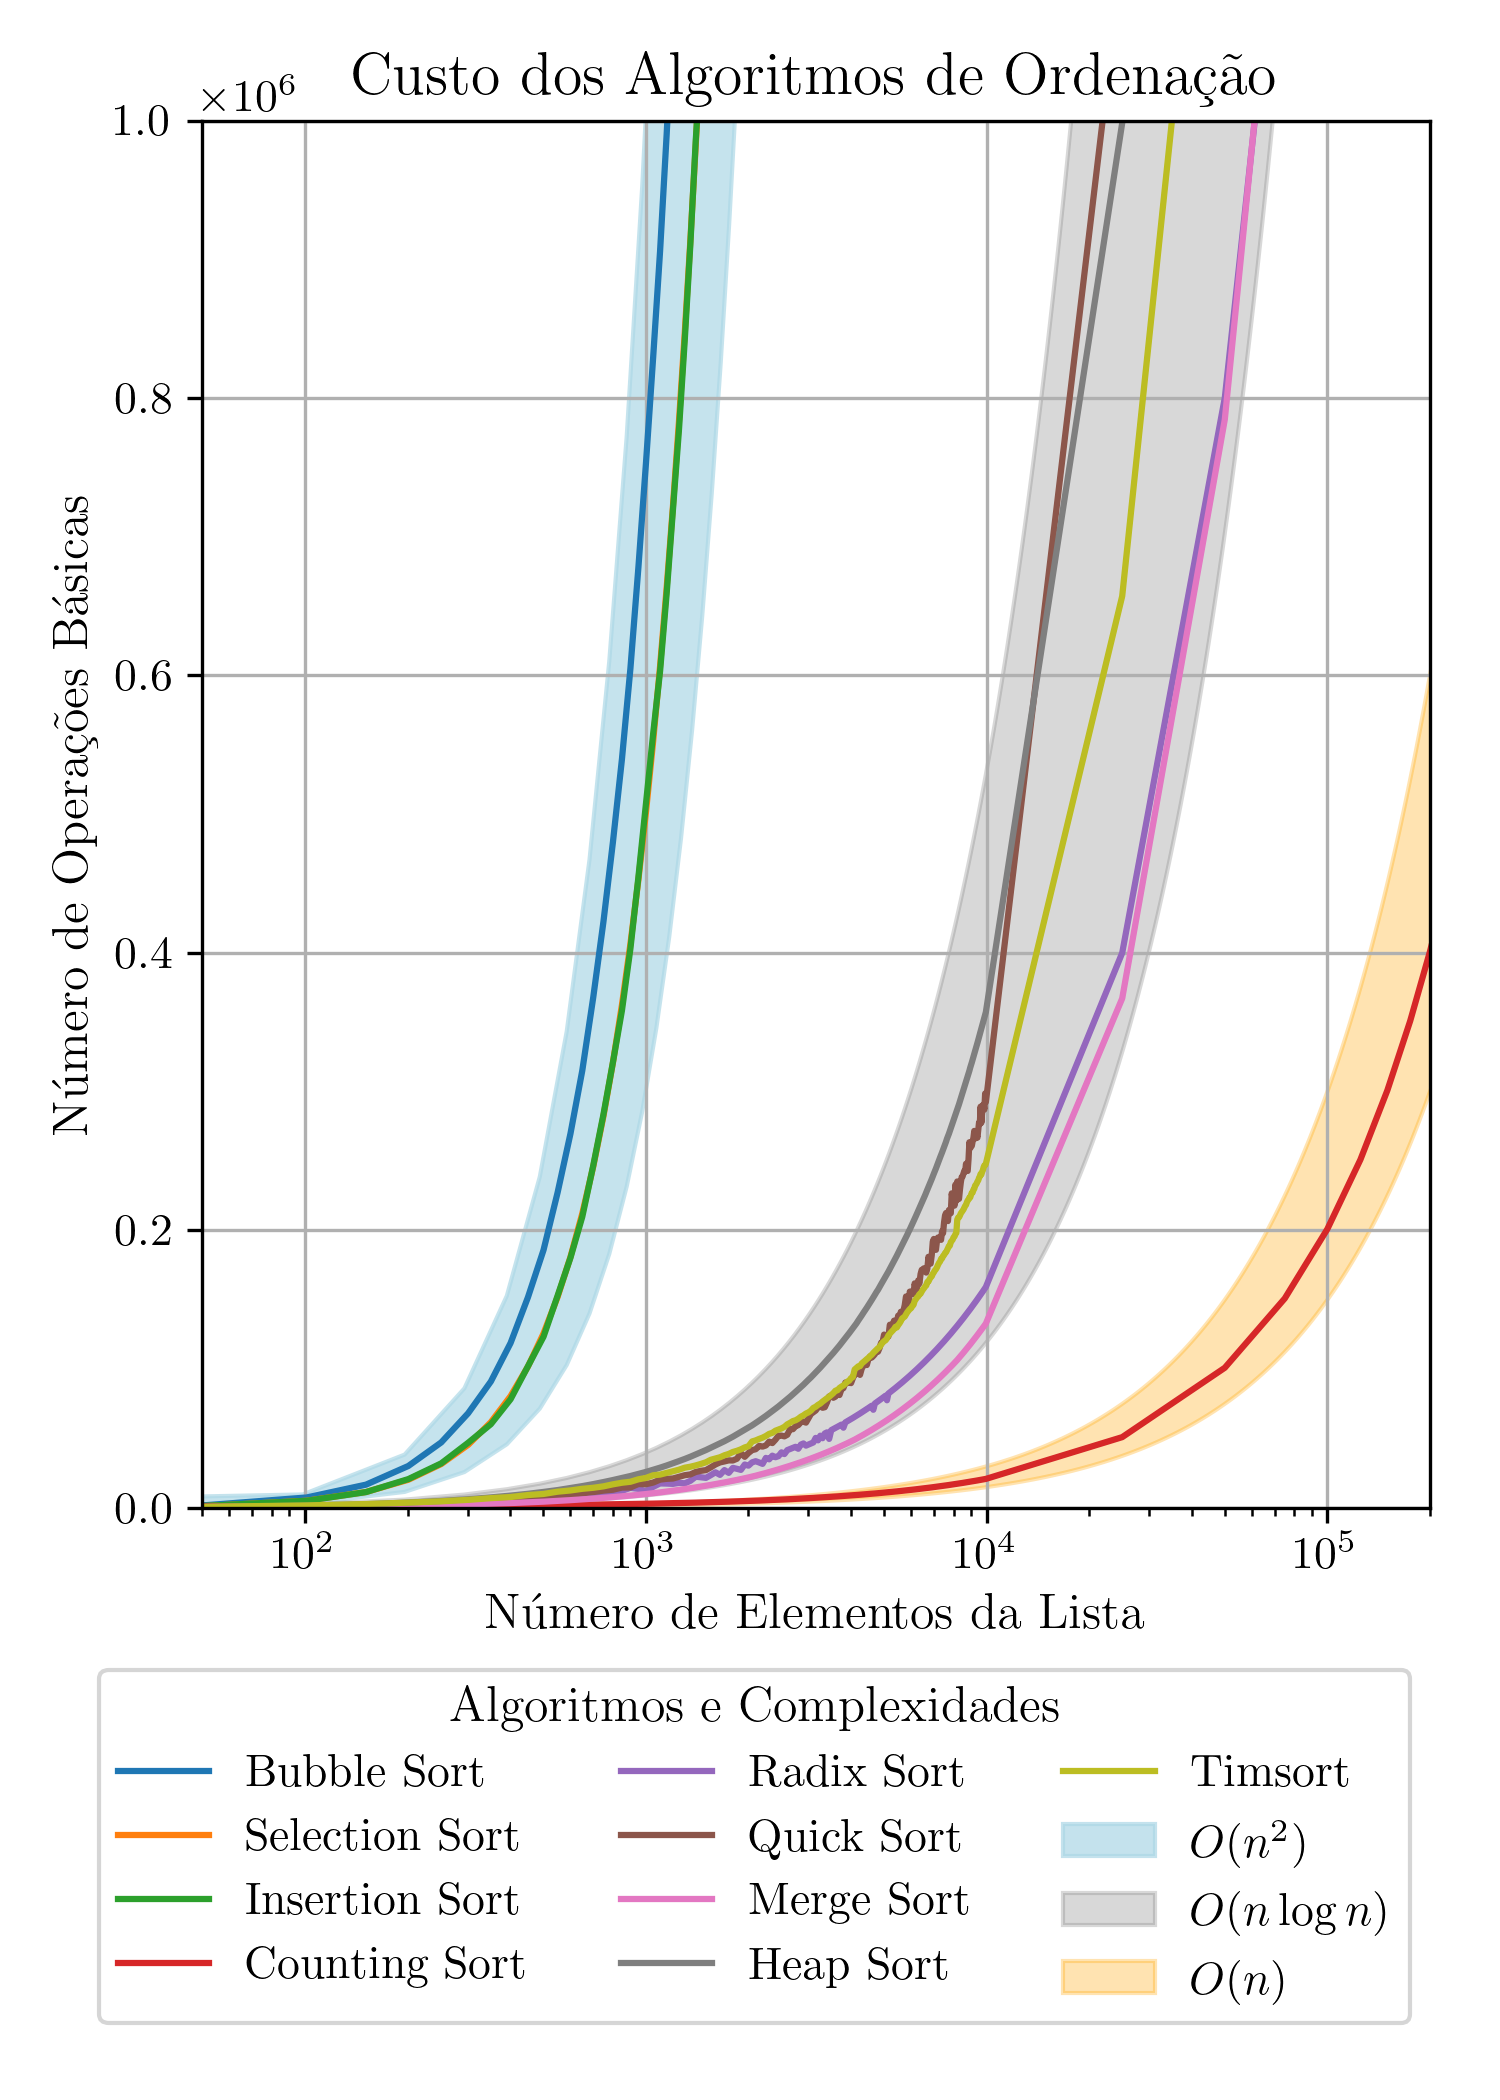
\includegraphics[width=1\linewidth]{sorting_complexities.png}
    \caption{Análise do número de operações básicas dos diferentes algoritmos face a diferentes tamanhos de listas.}
    \label{fig:sorting_complexities}
\end{figure}

A partir da análise da figura \ref{fig:sorting_complexities}, que contém os resultados práticos da implementação dos algoritmos analisados, torna-se possível então a comparação entre o comportamento empírico com a complexidade teórica.

No caso do Counting Sort, é possível verificar que a sua complexidade se comporta como \( \mathcal{O}(n) \), uma vez que o valor máximo presente na lista (\( k = 1000 \)) é significativamente menor do que os tamanhos das listas utilizadas nesta simulação. Assim, o termo adicional \( k \) não afeta substancialmente o crescimento do tempo de execução.

Relativamente aos algoritmos Bubble Sort, Selection Sort e Insertion Sort, observa-se um crescimento quadrático consistente com a complexidade teórica \( \mathcal{O}(n^2) \). Nota-se que o desempenho do Selection Sort não se destaca visualmente no gráfico, por se sobrepor ao do Insertion Sort, evidenciando o mesmo comportamento assintótico.

Quanto aos restantes algoritmos, com exceção do Radix Sort, todos apresentam um crescimento compatível com a complexidade \( \mathcal{O}(n \log n) \), conforme previsto teoricamente. Já o Radix Sort, cuja complexidade é dada por \( \mathcal{O}(n \cdot b) \), onde \( b \) representa o número de dígitos necessários para representar o maior valor \( k \), pode também ser expressa como \( \mathcal{O}(n \cdot \log_b k) \), assumindo uma base \( b \) fixa. Na representaçãos gráfica, observa-se que o seu desempenho tende a aproximar-se dos algoritmos de complexidade \( \mathcal{O}(n \log n) \), devido à presença de um fator logarítmico multiplicativo que, apesar de ser pequeno, afeta o crescimento linear.

Este resultado demonstra que, apesar das complexidades teóricas associadas a cada algoritmo, o seu desempenho prático depende fortemente das características da lista a ser ordenada, como a distribuição dos valores ou a presença de padrões específicos nos dados.

\section{Conclusão}

Neste trabalho, foram analisados e comparados nove algoritmos de ordenação, abrangendo abordagens clássicas (como Bubble Sort, Selection Sort e Insertion Sort), algoritmos mais eficientes baseados em paradigmas de dividir-para-conquistar (como Quick Sort, Merge Sort e Heap Sort), e algoritmos especializados como Counting Sort, Radix Sort e Timsort. Para cada algoritmo, foram descritos o funcionamento, a complexidade teórica, as vantagens e limitações, e o comportamento prático observado através de simulações em \textit{Python}.

A análise empírica permitiu confirmar, de forma geral, as previsões teóricas. Algoritmos quadráticos apresentaram um crescimento acentuado com o aumento do tamanho da lista, tornando-se inviáveis para grandes volumes de dados. Por outro lado, algoritmos com complexidade \( \mathcal{O}(n \log n) \) revelaram-se muito mais eficientes e escaláveis. O caso do Radix Sort destacou a importância de considerar não apenas a complexidade assintótica, mas também os fatores constantes ocultos e as condições específicas dos dados, uma vez que, apesar da sua complexidade quase linear, o seu desempenho prático aproxima-se frequentemente dos algoritmos \( \mathcal{O}(n \log n) \) devido ao custo das múltiplas passagens.

Conclui-se, assim, que a escolha do algoritmo de ordenação mais adequado não deve ser feita apenas com base na complexidade teórica, mas também considerando as características concretas dos dados, o contexto de utilização e os requisitos práticos de desempenho e memória.

\bibliographystyle{IEEEtran}
\bibliography{references}

\end{document}



